\documentclass[11pt,a4paper]{article}
\usepackage[utf8]{inputenc}
\usepackage[T1]{fontenc}
\usepackage[spanish,es-nodecimaldot,es-tabla]{babel}
\usepackage{lmodern,amsmath,amssymb,graphicx,pdfpages,booktabs,longtable,array,float,xcolor,listings,fancyhdr,titlesec,caption,needspace,microtype,xurl,hyperref}
\usepackage[top=2.3cm,bottom=2.3cm,left=2.2cm,right=2.2cm]{geometry}
\definecolor{azul}{HTML}{164769}
\definecolor{gris}{HTML}{F3F5F7}
\hypersetup{colorlinks=true,linkcolor=azul,urlcolor=azul,pdftitle={CVRP de logística urbana},pdfauthor={Equipo MA2015}}
\titleformat{\section}{\Large\bfseries}{\thesection.}{0.6em}{}
\titleformat{\subsection}{\large\bfseries}{\thesubsection.}{0.6em}{}
\titlespacing*{\section}{0pt}{16pt}{8pt}
\titlespacing*{\subsection}{0pt}{12pt}{6pt}
\setlength{\parindent}{0pt}\setlength{\parskip}{6pt}
\setlength{\emergencystretch}{2em}
\renewcommand{\arraystretch}{1.18}
\numberwithin{equation}{section}
\newcolumntype{P}[1]{>{\raggedright\arraybackslash}p{#1}}
\pagestyle{fancy}\fancyhf{}
\fancyhead[L]{\small Diseño de algoritmos matemáticos bioinspirados}
\fancyhead[R]{\small CVRP · Etapa 1}
\fancyfoot[C]{\thepage}\setlength{\headheight}{14pt}
\renewcommand{\headrulewidth}{0.3pt}
\captionsetup{font=small,labelfont=bf,justification=justified,singlelinecheck=false}
\lstset{basicstyle=\ttfamily\fontsize{8}{9.5}\selectfont,breaklines=true,columns=fullflexible,keepspaces=true,showstringspaces=false,frame=single,rulecolor=\color{black!18},backgroundcolor=\color{gris},xleftmargin=5pt,xrightmargin=5pt,framesep=5pt,tabsize=4,literate={á}{{\'a}}1 {é}{{\'e}}1 {í}{{\'i}}1 {ó}{{\'o}}1 {ú}{{\'u}}1 {ñ}{{\~n}}1 {ü}{{\"u}}1 {Ó}{{\'O}}1}
\begin{document}
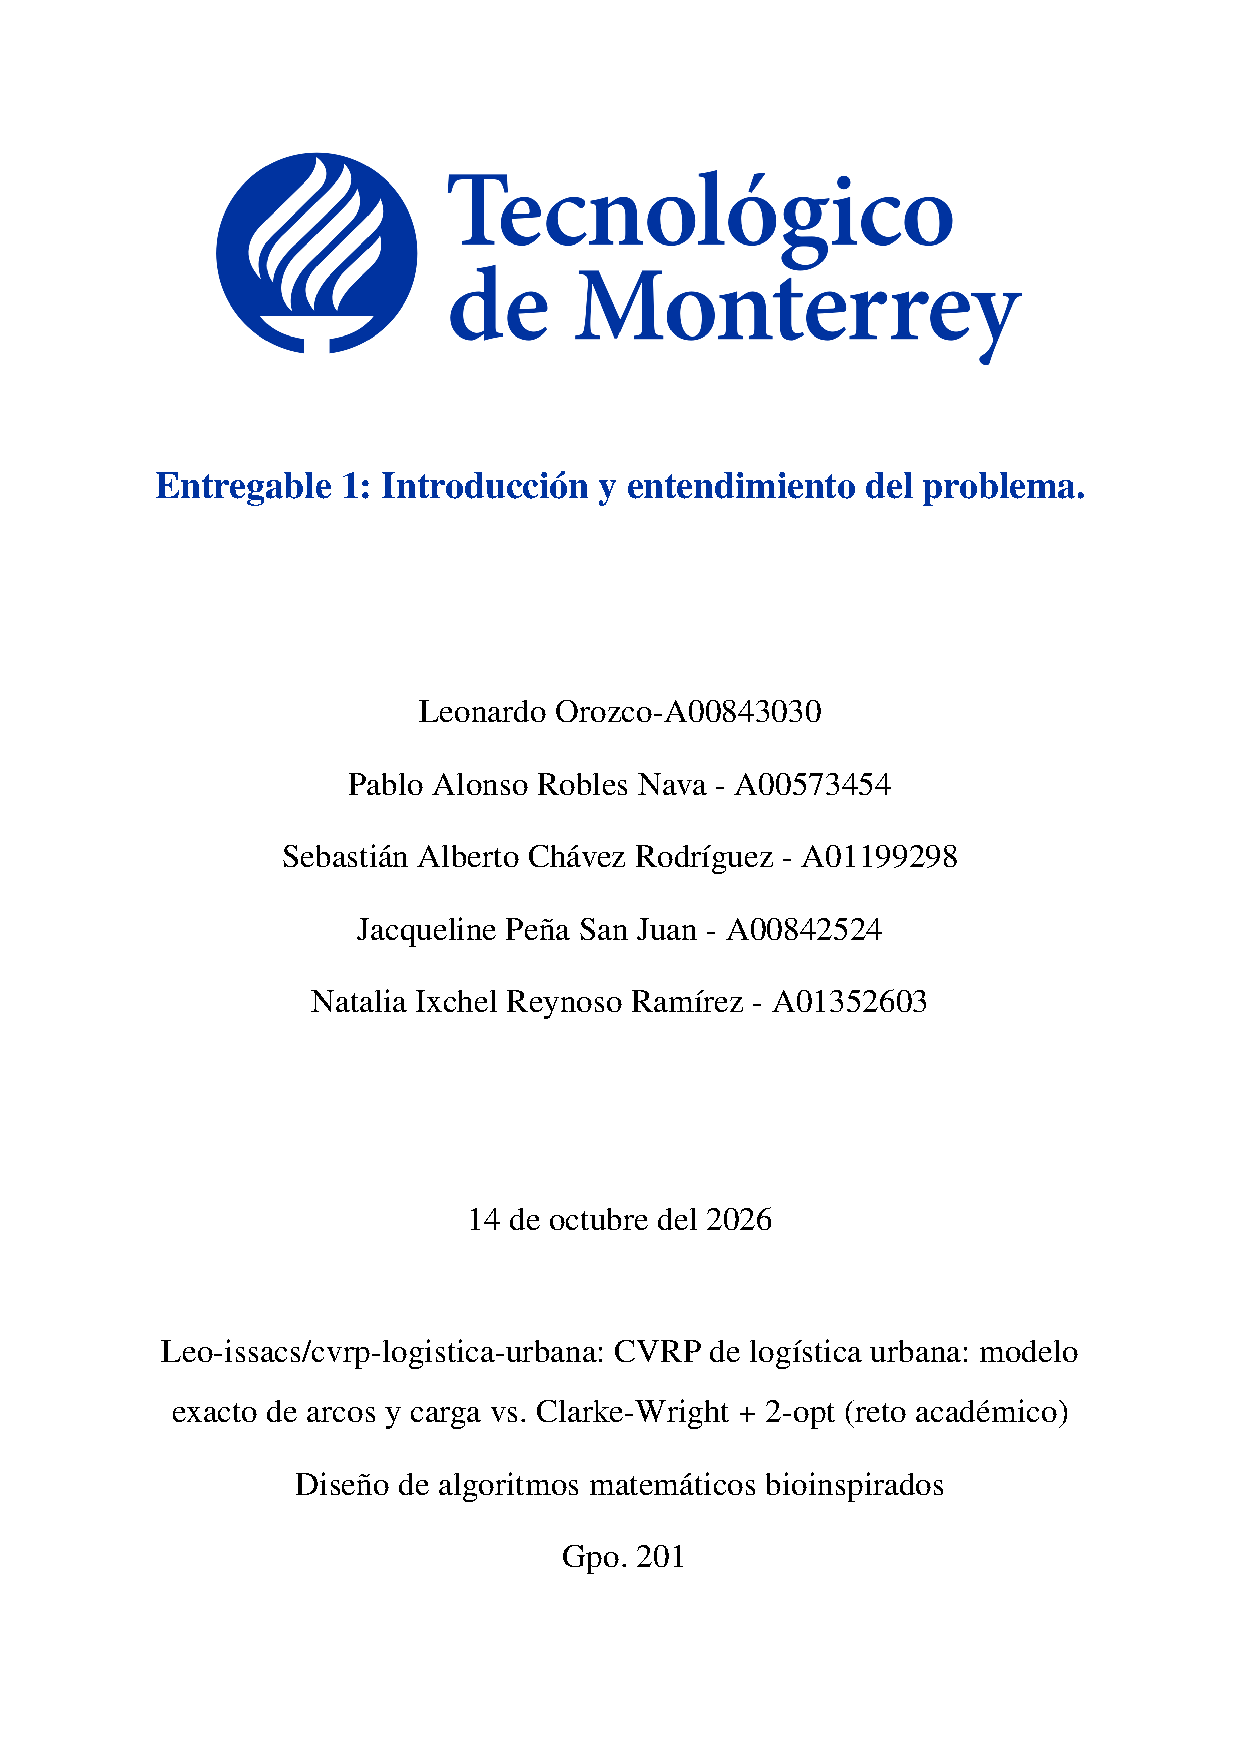
\includepdf[pages=1,fitpaper=true,pagecommand={\thispagestyle{empty}}]{portada_final.pdf}
\setcounter{page}{2}


\Needspace{110pt}

\section{Introducción y percepción inicial}

El crecimiento de las compras en línea exige distribuir numerosos pedidos en espacios urbanos limitados. La situación descrita por Sherman (2018) reúne dificultades de estacionamiento, congestión, costos de reparto y presión por entregar con rapidez. Nuestra percepción inicial es que mejorar las entregas requiere coordinar la asignación de clientes, el orden de visita y la carga de los vehículos. Este informe estudia esas decisiones mediante una instancia de diez clientes y compara una solución exacta con una heurística de ahorros y mejora local.


\Needspace{110pt}

\subsection{¿Qué es el CVRP?}

El problema de ruteo de vehículos con capacidad limitada (Capacitated Vehicle Routing Problem, CVRP) consiste en construir rutas que parten de un depósito, atienden la demanda de los clientes y regresan al mismo depósito. Cada cliente debe ser atendido una sola vez y la carga asignada a una ruta no puede exceder la capacidad del vehículo. El objetivo habitual es minimizar la distancia o el costo total de los recorridos. La asignación de clientes combina una decisión de agrupamiento por capacidad con una decisión sobre el orden de visita; por ello, se relaciona tanto con el empaquetamiento como con el problema del agente viajero (Orrego Cardozo et al., 2016).


En este trabajo se estudia un CVRP estático, determinista, simétrico y con flota homogénea. Se conocen todas las demandas antes de planear; no se permiten entregas divididas ni recargas intermedias. El archivo no especifica una flota fija, horarios ni costos monetarios. Por tanto, el caso principal minimiza la distancia y deja que el modelo determine cuántas rutas usar. Además se evalúa el escenario con tres rutas para distinguir la flota mínima de la solución de menor recorrido.


\Needspace{110pt}

\subsection{Costos logísticos del reparto}

El costo de última milla combina el uso de vehículos, combustible, mantenimiento, trabajo del conductor, servicio, búsqueda de estacionamiento y reintentos de entrega. McKinsey \& Company (2016, p. 6) señala que esta etapa frecuentemente alcanza o supera el 50\% del costo total de entrega de paquetes, lo que explica el interés por mejorar su planificación.


La distancia representa sólo una parte del costo. McKinsey \& Company (2018) estima que, en redes densas, el costo total del vehículo, incluido el kilometraje, supone menos del 15\% del costo de última milla. Por su parte, Dalla Chiara y Goodchild (2020) analizaron 2,900 trayectos de reparto y recolección en el centro de Seattle y estimaron 2.3 minutos de búsqueda de estacionamiento por trayecto, equivalentes al 28\% de su tiempo total. Estos resultados muestran la importancia de considerar también la flota, el servicio y las condiciones de operación.


Un marco para evaluar el costo logístico es


\begin{equation}\label{eq:costo}
C_{\mathrm{log}}=F m+aD+bT+P
\end{equation}


donde F representa el costo fijo por vehículo, m el número de rutas, a el costo por unidad de distancia, D la distancia total, b el costo laboral por unidad de tiempo, T el tiempo operativo y P los cargos por estacionamiento o reintentos. Los componentes se definen de forma complementaria para evitar contabilizar dos veces un mismo gasto.

Con las coordenadas, demandas y capacidad disponibles, este estudio minimiza la distancia D. La comparación entre tres y cuatro rutas permite interpretar su relación con el costo: tres rutas recorren 20.175187 unidades adicionales. Manteniendo iguales los demás componentes, esa opción sería preferible si el ahorro de un vehículo superara el costo del recorrido adicional, es decir, si \(F>a\cdot20.175187\).


\Needspace{110pt}

\subsection{Impacto ambiental y reparto urbano}

El reparto urbano genera circulación adicional para buscar estacionamiento, paradas frecuentes y consumo energético durante la circulación y la espera. Estas operaciones relacionan el ruteo con las emisiones, la congestión y la ocupación del espacio vial. En su escenario de no intervención para las 100 ciudades más grandes, el World Economic Forum (2020) proyectó hacia 2030 un aumento del 36\% en los vehículos de reparto y de alrededor de un tercio en las emisiones asociadas, hasta 25 millones de toneladas de CO\textsubscript{2} anuales.


El mismo análisis evaluó una combinación de electrificación, entregas fuera de horas pico, consolidación de cargas, casilleros y ruteo dinámico: estimó reducciones de aproximadamente 30\% en CO\textsubscript{2} y congestión y de 25\% en costos de entrega frente a su escenario de no intervención para 2030 (World Economic Forum, 2020). La interpretación es que la optimización de rutas debe coordinarse con decisiones de flota y operación; cambiar únicamente el vehículo no elimina los recorridos ni la ocupación de la calle.


Bekta\c{s} y Laporte (2011) incorporan carga y velocidad al consumo energético; Zhang et al. (2015) integran combustible, carbono y uso de vehículos. Su aportación al reto es concreta: dos recorridos de igual longitud pueden tener emisiones diferentes si cambian la carga, velocidad, tecnología o tiempo de espera. Para una futura extensión se requerirían distancias reales, consumo por tramo, combustible o electricidad utilizada y factores de emisión con un alcance definido, por ejemplo emisiones de operación frente a ciclo de vida.


La solución exacta reduce el recorrido en 20.263383 unidades frente a la heurística, equivalentes al 5.97\% de la distancia heurística. Bajo una tasa constante de emisiones por unidad de distancia, esa reducción se traduciría proporcionalmente al componente de emisiones por recorrido. Una evaluación ambiental completa deberá incorporar además carga, velocidad, tecnología y espera, como proponen los trabajos citados.


\Needspace{110pt}

\subsection{Objetivo y alcance}

Caracterizar el reparto urbano mediante un CVRP de diez clientes y comparar una solución exacta con una heurística reproducible. Se busca construir la matriz de distancias, formular las decisiones y restricciones, obtener rutas factibles, medir su utilización de capacidad y evaluar la diferencia porcentual de distancia y tiempo. El análisis también identifica qué información adicional permitiría incorporar congestionamiento, ventanas de entrega y criterios ambientales en etapas posteriores.


\Needspace{110pt}

\section{Trabajo relacionado}

La Tabla~\ref{tab:1} compara siete artículos sobre ruteo capacitado y sus extensiones ambientales. Se distinguen el problema, el método de solución y su utilidad para el caso estudiado.


\Needspace{130pt}

{\small\begin{longtable}{P{\dimexpr 0.17\linewidth-8.16pt\relax}P{\dimexpr 0.19\linewidth-9.120000000000001pt\relax}P{\dimexpr 0.28\linewidth-13.440000000000001pt\relax}P{\dimexpr 0.36\linewidth-17.28pt\relax}}

\caption{Comparación de literatura científica.}\label{tab:1}\\

\toprule

\textbf{Artículo} & \textbf{Problema} & \textbf{Método} & \textbf{Aplicación y límite en este reto}\\\midrule

\endfirsthead

\caption[]{Comparación de literatura científica. (continuación)}\\

\toprule

\textbf{Artículo} & \textbf{Problema} & \textbf{Método} & \textbf{Aplicación y límite en este reto}\\\midrule

\endhead

\bottomrule\endfoot

Clarke y Wright (1964) & Distribución desde un depósito; capacidad & Heurística de ahorros & Construye rutas por fusiones; base del algoritmo utilizado, sin garantía de optimalidad.\\[2pt]

Gillett y Miller (1974) & Ruteo con carga y distancia limitadas & Barrido angular y mejora & Separa agrupación y secuenciación; depende del orden angular.\\[2pt]

Prins (2004) & CVRP & Algoritmo genético híbrido y división de rutas & Combina permutaciones y búsqueda local; la división óptima depende del orden del cromosoma.\\[2pt]

Orrego Cardozo et al. (2016) & CVRP & Barrido y genético Chu--Beasley modificado & Antecedente bioinspirado en español; no equivale a la heurística ejecutada aquí.\\[2pt]

Vidal (2022) & CVRP & Búsqueda genética híbrida y SWAP* & Permite intercambios entre rutas; referencia para superar la asignación fija de 2-opt.\\[2pt]

Bekta\c{s} y Laporte (2011) & Pollution-Routing Problem & Modelación de velocidad, carga y emisiones & Relaciona ruteo y energía; necesita parámetros físicos ausentes en la instancia.\\[2pt]

Zhang et al. (2015) & Ruteo con combustible y carbono & Búsqueda tabú mejorada RS-TS & Integra flota y emisiones; exige calibrar costos antes de trasladarlos al caso.\\[2pt]

\end{longtable}}

La literatura sugiere comenzar con una referencia exacta y una heurística transparente, y después estudiar métodos bioinspirados para instancias mayores. En particular, los enfoques genéticos combinados con mejora local trabajan tanto la asignación como el orden de visita. La elección final debe depender del tamaño, las restricciones y el tiempo disponible, y no sólo del nombre del algoritmo.


Toth y Vigo (eds., 2014) complementan estos artículos con una exposición de métodos exactos de ramificación y acotamiento, generación de columnas y cortes para el CVRP. Esta referencia sitúa la formulación por arcos y carga dentro de una familia más amplia de métodos de optimización.


\Needspace{110pt}

\section{Datos y matriz de costos}

La instancia CVRP\_10 contiene once nodos: el depósito 1 y los diez clientes 2 a 11. La capacidad por vehículo es Q = 50 y la demanda total es 146 unidades. Las coordenadas y demandas se presentan en la Tabla~\ref{tab:2}; sus magnitudes se expresan en unidades de distancia y de carga.


\Needspace{300pt}

{\small\begin{longtable}{P{\dimexpr 0.12\linewidth-7.199999999999999pt\relax}P{\dimexpr 0.17\linewidth-10.2pt\relax}P{\dimexpr 0.17\linewidth-10.2pt\relax}P{\dimexpr 0.22\linewidth-13.200000000000001pt\relax}P{\dimexpr 0.32\linewidth-19.2pt\relax}}

\caption{Coordenadas y demanda.}\label{tab:2}\\

\toprule

\textbf{Nodo} & \textbf{x} & \textbf{y} & \textbf{Demanda} & \textbf{Tipo}\\\midrule

\endfirsthead

\caption[]{Coordenadas y demanda. (continuación)}\\

\toprule

\textbf{Nodo} & \textbf{x} & \textbf{y} & \textbf{Demanda} & \textbf{Tipo}\\\midrule

\endhead

\bottomrule\endfoot

1 & 50 & 50 & 0 & Depósito\\[2pt]

2 & 20 & 70 & 12 & Cliente\\[2pt]

3 & 30 & 80 & 18 & Cliente\\[2pt]

4 & 60 & 75 & 10 & Cliente\\[2pt]

5 & 80 & 70 & 15 & Cliente\\[2pt]

6 & 25 & 45 & 14 & Cliente\\[2pt]

7 & 40 & 30 & 20 & Cliente\\[2pt]

8 & 65 & 25 & 16 & Cliente\\[2pt]

9 & 85 & 40 & 11 & Cliente\\[2pt]

10 & 45 & 60 & 13 & Cliente\\[2pt]

11 & 70 & 55 & 17 & Cliente\\[2pt]

\end{longtable}}

\Needspace{110pt}

\subsection{Convención de distancia}


\begin{equation}\label{eq:distancia}
c_{ij}=\sqrt{(X_i-X_j)^2+(Y_i-Y_j)^2},\qquad c_{ii}=0,\quad c_{ij}=c_{ji}
\end{equation}


Los cálculos principales emplean distancias euclidianas sin redondear. La Tabla~\ref{tab:3} muestra dos decimales para facilitar la lectura; el modelo conserva la precisión completa. Por ejemplo, \(c_{12}=\sqrt{(50-20)^2+(50-70)^2}=\sqrt{1300}\approx36.05551275\).


El identificador EUC\_2D del archivo corresponde a la convención TSPLIB de redondeo al entero más cercano (Reinelt, 1991; TSPLIB FAQ). Para estudiar la distancia geométrica se adopta aquí la variante euclidiana continua. Como comprobación de sensibilidad, la variante entera, calculada con floor(distancia + 0.5), tiene óptimo 317 y conserva los cuatro grupos de clientes. La diferencia entre ambos valores responde a la matriz de costos utilizada.


\Needspace{130pt}

\begin{table}[H]\centering

\caption{Matriz de distancias euclidianas (dos decimales).}\label{tab:3}

\setlength{\tabcolsep}{3pt}\resizebox{\linewidth}{!}{\begin{tabular}{rrrrrrrrrrrr}

\toprule

\textbf{i / j} & \textbf{1} & \textbf{2} & \textbf{3} & \textbf{4} & \textbf{5} & \textbf{6} & \textbf{7} & \textbf{8} & \textbf{9} & \textbf{10} & \textbf{11}\\\midrule

1 & 0.00 & 36.06 & 36.06 & 26.93 & 36.06 & 25.50 & 22.36 & 29.15 & 36.40 & 11.18 & 20.62\\

2 & 36.06 & 0.00 & 14.14 & 40.31 & 60.00 & 25.50 & 44.72 & 63.64 & 71.59 & 26.93 & 52.20\\

3 & 36.06 & 14.14 & 0.00 & 30.41 & 50.99 & 35.36 & 50.99 & 65.19 & 68.01 & 25.00 & 47.17\\

4 & 26.93 & 40.31 & 30.41 & 0.00 & 20.62 & 46.10 & 49.24 & 50.25 & 43.01 & 21.21 & 22.36\\

5 & 36.06 & 60.00 & 50.99 & 20.62 & 0.00 & 60.42 & 56.57 & 47.43 & 30.41 & 36.40 & 18.03\\

6 & 25.50 & 25.50 & 35.36 & 46.10 & 60.42 & 0.00 & 21.21 & 44.72 & 60.21 & 25.00 & 46.10\\

7 & 22.36 & 44.72 & 50.99 & 49.24 & 56.57 & 21.21 & 0.00 & 25.50 & 46.10 & 30.41 & 39.05\\

8 & 29.15 & 63.64 & 65.19 & 50.25 & 47.43 & 44.72 & 25.50 & 0.00 & 25.00 & 40.31 & 30.41\\

9 & 36.40 & 71.59 & 68.01 & 43.01 & 30.41 & 60.21 & 46.10 & 25.00 & 0.00 & 44.72 & 21.21\\

10 & 11.18 & 26.93 & 25.00 & 21.21 & 36.40 & 25.00 & 30.41 & 40.31 & 44.72 & 0.00 & 25.50\\

11 & 20.62 & 52.20 & 47.17 & 22.36 & 18.03 & 46.10 & 39.05 & 30.41 & 21.21 & 25.50 & 0.00\\

\bottomrule\end{tabular}}

\end{table}

\Needspace{110pt}

\section{Definición y modelo matemático}

\Needspace{110pt}

\subsection{Grafo, decisiones y supuestos}

Sea \(G=(V,A)\) un grafo dirigido completo sin lazos. \(V=\{1,\ldots,11\}\) contiene el depósito 1 y \(C=V\setminus\{1\}=\{2,\ldots,11\}\) contiene los diez clientes; \(A=\{(i,j):i,j\in V,\ i\ne j\}\) contiene 110 arcos. Aunque se usan arcos dirigidos para expresar el orden de visita, la matriz es simétrica: \(c_{ij}\) = \(c_{ji}\). Cada cliente tiene demanda conocida \(q_i\) > 0, el depósito tiene \(q_1\) = 0 y la capacidad homogénea es Q = 50.


Se decide qué arcos recorrer y cuánta carga transportar en ellos, de modo que cada cliente reciba su demanda completa una vez y cada vehículo salga del depósito y regrese a él. Cada ruta corresponde a una salida de un vehículo, sin entregas divididas ni recargas intermedias. El objetivo minimiza la distancia total y determina el número de rutas. Después se analiza una flota de exactamente tres vehículos.


\Needspace{350pt}

\subsection{Conjuntos, parámetros y variables}

\Needspace{260pt}

{\small\begin{longtable}{P{\dimexpr 0.26\linewidth-6.24pt\relax}P{\dimexpr 0.74\linewidth-17.759999999999998pt\relax}}

\caption{Elementos de la formulación explícita.}\label{tab:4}\\

\toprule

\textbf{Símbolo} & \textbf{Tipo y significado}\\\midrule

\endfirsthead

\caption[]{Elementos de la formulación explícita. (continuación)}\\

\toprule

\textbf{Símbolo} & \textbf{Tipo y significado}\\\midrule

\endhead

\bottomrule\endfoot

V, C, A & Conjuntos de nodos, clientes y arcos dirigidos. El nodo 1 es el depósito.\\[2pt]

\(q_i\); Q = 50 & Parámetros: demanda del nodo i y capacidad por vehículo; \(q_1\) = 0.\\[2pt]

\(c_{ij}\) & Parámetro: distancia euclidiana sin redondear del nodo i al j.\\[2pt]

\(x_{ij}\in\{0,1\}\) & Variable binaria: vale 1 si se recorre el arco i \(\to\) j, y 0 en caso contrario.\\[2pt]

\(f_{ij}\ge0\) & Variable continua: carga física a bordo durante el arco i \(\to\) j, después de atender i y antes de atender j.\\[2pt]

\(m=\sum_{j\in C}x_{1j}\) & Expresión entera: número de salidas del depósito y, por tanto, de rutas utilizadas.\\[2pt]

\(S\subseteq C\) & Subconjunto no vacío de clientes utilizado en la demostración de conectividad.\\[2pt]

\(Z;L_r;U_r\) & Resultados derivados: distancia total, carga inicial de una ruta y porcentaje de capacidad no utilizada.\\[2pt]

\end{longtable}}

\Needspace{110pt}

\subsection{Función objetivo y restricciones}

Se emplea una formulación de arcos y flujo de producto. Las variables \(x_{ij}\) seleccionan los recorridos y \(f_{ij}\) representan la carga transportada. Las ecuaciones \eqref{eq:m1}--\eqref{eq:m7} y los dominios \eqref{eq:m9} describen el modelo; la expresión \eqref{eq:m8} demuestra su conectividad. Todas las sumas sobre arcos excluyen i = j.



\begin{equation}\label{eq:m1}
\min\quad Z=\sum_{(i,j)\in A}c_{ij}x_{ij}
\end{equation}


Minimizar la distancia total de los arcos seleccionados.



\begin{equation}\label{eq:m2}
\sum_{j\in V\setminus\{i\}}x_{ji}=1,\qquad i\in C
\end{equation}


Cada cliente recibe una única visita.



\begin{equation}\label{eq:m3}
\sum_{j\in V\setminus\{i\}}x_{ij}=\sum_{j\in V\setminus\{i\}}x_{ji},\qquad i\in C
\end{equation}


Conservación del recorrido: por cada llegada hay una salida.



\begin{equation}\label{eq:m4}
m=\sum_{j\in C}x_{1j}=\sum_{i\in C}x_{i1},\qquad \left\lceil\frac{\sum_{i\in C}q_i}{Q}\right\rceil\le m\le |C|
\end{equation}


Salidas y regresos al depósito; cota inferior de rutas.



\begin{equation}\label{eq:m5}
\sum_{j\in V\setminus\{i\}}f_{ji}-\sum_{j\in V\setminus\{i\}}f_{ij}=q_i,\qquad i\in C
\end{equation}


Balance de producto: carga que llega menos carga que sale igual a la entrega.



\begin{equation}\label{eq:m6}
0\le f_{ij}\le Qx_{ij},\qquad(i,j)\in A
\end{equation}


Capacidad y vínculo entre carga y recorrido; sin arco no se transporta producto.



\begin{equation}\label{eq:m7}
f_{i1}=0\ (i\in C),\qquad\sum_{j\in C}f_{1j}=\sum_{i\in C}q_i=146
\end{equation}


Regreso vacío y carga total despachada desde el depósito.



\begin{equation}\label{eq:m8}
\emptyset\ne S\subseteq C\text{ aislado}\quad\Longrightarrow\quad 0=\sum_{i\in S}q_i>0
\end{equation}


Contradicción que excluye ciclos aislados: consecuencia de \eqref{eq:m5} y \eqref{eq:m6}, no una restricción adicional.



\begin{equation}\label{eq:m9}
x_{ij}\in\{0,1\},\qquad f_{ij}\in\mathbb{R}_{\ge0},\qquad(i,j)\in A
\end{equation}


Dominio binario del recorrido y no negatividad de la carga.


Las restricciones \eqref{eq:m2} y \eqref{eq:m3} obligan a entrar y salir una vez de cada cliente. La ecuación \eqref{eq:m4} equilibra el depósito; su cota inferior se deriva de la demanda total, pero no obliga a usar exactamente tres vehículos. Para evaluar ese escenario se agrega m = 3. La ecuación \eqref{eq:m5} descuenta \(q_i\) unidades al atender i, mientras que \eqref{eq:m6} limita la carga de cualquier vehículo a 50. La ecuación \eqref{eq:m7} fija una operación de entregas puras: se despachan exactamente 146 unidades y los vehículos regresan sin producto.


El flujo de producto garantiza la conexión con el depósito. Si un conjunto no vacío S de clientes quedara aislado, la restricción \eqref{eq:m6} impediría cualquier flujo de carga a través de su frontera. Al sumar los balances \eqref{eq:m5}, los flujos internos se cancelarían y se obtendría \eqref{eq:m8}, una contradicción porque \(q_i\) > 0 para todos los clientes. Por tanto, cada ruta queda conectada con el depósito.


La implementación contiene 110 variables binarias, 110 continuas y 154 restricciones. Fijar m = 3 añade una restricción. La carga total despachada y la cota m \(\le\) 10 se deducen de los balances y de las visitas; se incluyen explícitamente para facilitar la interpretación. La cota m \(\ge\) 3 incorpora la capacidad total requerida.


\Needspace{110pt}

\subsection{Relación entre variables, acciones y restricciones}

La Figura~\ref{fig:1} relaciona las variables de recorrido y carga con las acciones de transporte y entrega y con las restricciones que las regulan. Se utiliza una de las rutas óptimas para mostrar cómo disminuye la carga al atender a cada cliente.


\begin{figure}[H]\centering

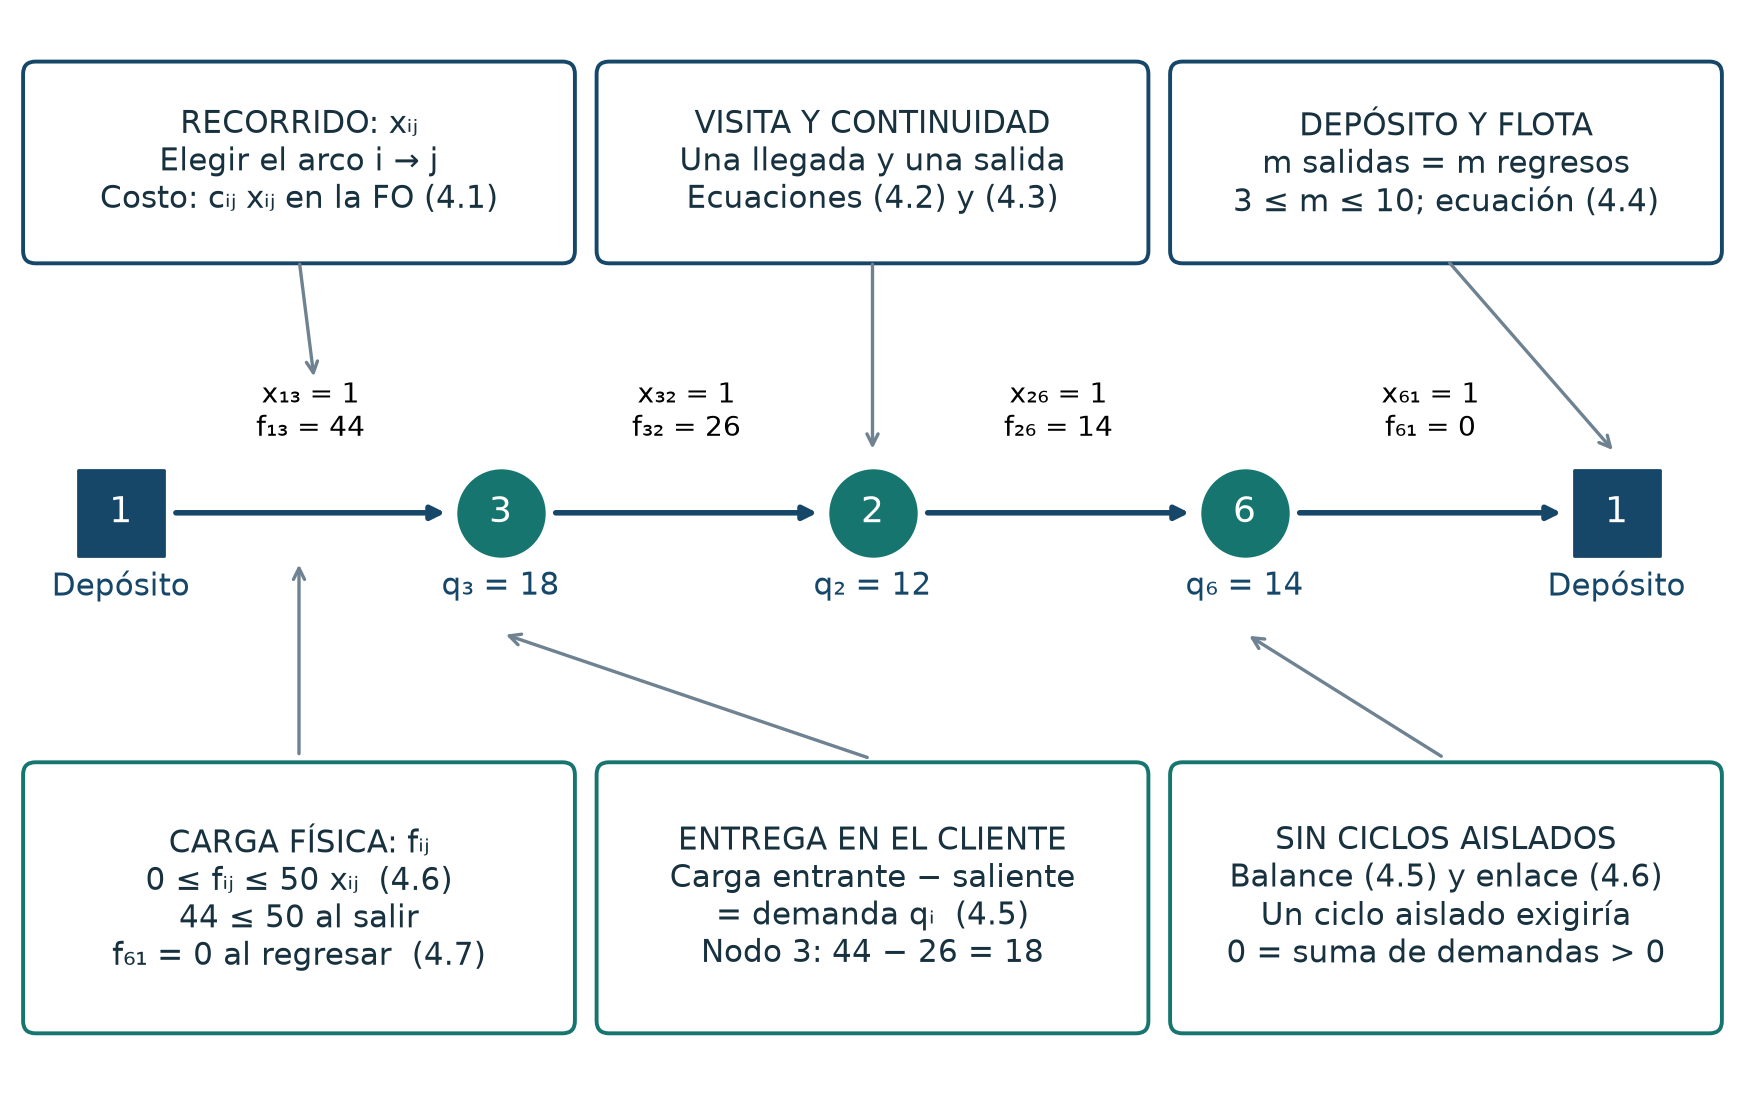
\includegraphics[width=1\linewidth,height=0.43\textheight,keepaspectratio]{figuras/diagrama.png}

\caption{Relación entre variables, acciones y restricciones en la ruta 1 \(\to\) 3 \(\to\) 2 \(\to\) 6 \(\to\) 1.}\label{fig:1}

\end{figure}

En la ruta ilustrada, \(x_{13}=x_{32}=x_{26}=x_{61}=1\). La carga parte con 44 unidades y disminuye a 26 después de atender al cliente 3, a 14 después del cliente 2 y a cero después del cliente 6. Cada diferencia coincide con la demanda entregada y la carga permanece por debajo de Q = 50. El diagrama muestra así la relación entre selección de arcos, continuidad, capacidad y balance de producto.


\Needspace{110pt}

\subsection{Implementación y comprobación}

El modelo se implementó en Python con PuLP 3.3.0 y se resolvió mediante CBC 2.10.3. La optimalidad se comprobó con el estado de terminación del solver y se verificaron la cobertura de clientes, la capacidad y el regreso al depósito. Una programación dinámica por particiones proporcionó una certificación independiente de los dos escenarios.


\Needspace{110pt}

\section{Algoritmo heurístico}

Se adopta el algoritmo de ahorros de Clarke--Wright con mejora 2-opt dentro de cada ruta. Esta heurística clásica construye una solución factible con rapidez y permite evaluar el intercambio entre calidad y tiempo frente al método exacto. Su pseudocódigo, implementación y resultados se presentan a continuación.



\begin{equation}\label{eq:ahorro}
s_{ij}=c_{1i}+c_{1j}-c_{ij}
\end{equation}


Inicialmente cada cliente tiene una ruta individual 1 \(\to\) i \(\to\) 1. Los pares se ordenan por ahorro decreciente. Se fusionan dos rutas distintas sólo si los clientes del par están en sus extremos y su demanda conjunta no supera 50. Los empates se resuelven por identificador de cliente ascendente. Después, 2-opt invierte segmentos internos cuando disminuye la distancia, hasta que ninguna inversión la mejora. Como esa mejora no mueve clientes entre rutas, conserva la factibilidad y puede quedar atrapada en una asignación poco conveniente.


\Needspace{250pt}

\subsection{Pseudocódigo}

\begin{minipage}{\linewidth}

\begin{lstlisting}

Entrada: clientes C, demandas q, capacidad Q y matriz c
Crear una ruta [1,i,1] por cliente i
Calcular s(i,j) = c(1,i) + c(1,j) - c(i,j)
Ordenar pares por ahorro decreciente y luego por (i,j)
Para cada par (i,j) con ahorro positivo:
    Identificar las rutas A y B que contienen i y j
    Si A != B, i y j son extremos y carga(A)+carga(B) <= Q:
        Orientar A para terminar en i y B para iniciar en j
        Fusionar A y B
Para cada ruta resultante:
    Mientras exista una inversión 2-opt que reduzca su distancia:
        Aplicar la mejor inversión factible
Verificar cobertura única, regreso al depósito y capacidad
Devolver rutas, distancia total y utilización de capacidad

\end{lstlisting}

\end{minipage}

\Needspace{110pt}

\section{Resultados y trazado de rutas}

\Needspace{110pt}

\subsection{Solución exacta del caso principal}

La solución exacta alcanza \(Z^*\) = 318.989487 unidades con cuatro rutas. CBC probó su optimalidad en las diez ejecuciones y la certificación por programación dinámica coincidió con este valor. La Tabla~\ref{tab:5} presenta los recorridos, cargas y capacidad no utilizada.


\Needspace{130pt}

{\small\begin{longtable}{P{\dimexpr 0.07\linewidth-4.2pt\relax}P{\dimexpr 0.4\linewidth-24.000000000000004pt\relax}P{\dimexpr 0.19\linewidth-11.400000000000002pt\relax}P{\dimexpr 0.16\linewidth-9.6pt\relax}P{\dimexpr 0.18\linewidth-10.8pt\relax}}

\caption{Rutas óptimas de distancia mínima.}\label{tab:5}\\

\toprule

\textbf{Ruta} & \textbf{Recorrido} & \textbf{Distancia} & \textbf{Carga / 50} & \textbf{No utilizado}\\\midrule

\endfirsthead

\caption[]{Rutas óptimas de distancia mínima. (continuación)}\\

\toprule

\textbf{Ruta} & \textbf{Recorrido} & \textbf{Distancia} & \textbf{Carga / 50} & \textbf{No utilizado}\\\midrule

\endhead

\bottomrule\endfoot

R1 & 1 \(\to\) 10 \(\to\) 1 & 22.361 & 13 & 74\%\\[2pt]

R2 & 1 \(\to\) 3 \(\to\) 2 \(\to\) 6 \(\to\) 1 & 101.188 & 44 & 12\%\\[2pt]

R3 & 1 \(\to\) 4 \(\to\) 5 \(\to\) 11 \(\to\) 1 & 86.185 & 42 & 16\%\\[2pt]

R4 & 1 \(\to\) 7 \(\to\) 8 \(\to\) 9 \(\to\) 1 & 109.256 & 47 & 6\%\\[2pt]

\end{longtable}}


\begin{equation}\label{eq:zopt}
\begin{aligned}Z^*&=22.360680+101.187844+86.184637+109.256327\\&=318.989487.\end{aligned}
\end{equation}



\begin{equation}\label{eq:capacidadlibre}
U_r=100\,\frac{Q-L_r}{Q},\qquad L_r=\sum_{i\text{ atendido en }r}q_i
\end{equation}


Las cuatro rutas ofrecen una capacidad conjunta de 200 unidades y transportan 146: la utilización global es 73\% y la capacidad no utilizada es 27\%. En la Figura~\ref{fig:2} se distinguen tres grupos de clientes y una ruta corta para el cliente 10. Aunque esa ruta aprovecha sólo el 26\% de su capacidad, permite reducir la distancia total; forzar su integración en otro recorrido altera las asignaciones óptimas.


\begin{figure}[H]\centering

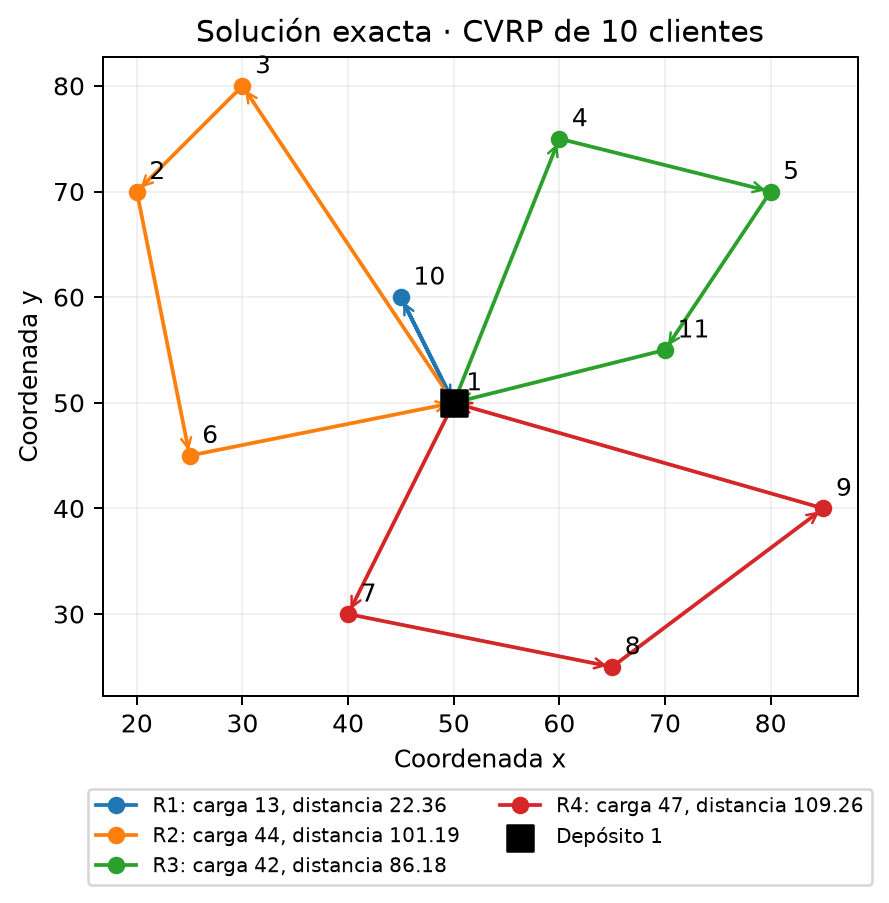
\includegraphics[width=0.82\linewidth,height=0.43\textheight,keepaspectratio]{figuras/rutas_exactas.png}

\caption{Rutas de distancia mínima. Las flechas indican el sentido de visita y el cuadrado representa el depósito.}\label{fig:2}

\end{figure}

\Needspace{110pt}

\subsection{Número mínimo de rutas y escenario de tres vehículos}


\begin{equation}\label{eq:flotaminima}
m\ge\left\lceil\frac{146}{50}\right\rceil=3
\end{equation}


La cota de capacidad establece un mínimo de tres rutas. Al imponer m = 3, el modelo obtiene \(Z_3\) = 339.164674 unidades, con optimalidad probada en las diez ejecuciones y confirmada por programación dinámica. La Tabla~\ref{tab:6} y la Figura~\ref{fig:3} muestran una solución óptima para este escenario.


Las cargas de 47, 50 y 49 unidades confirman que tres vehículos son suficientes. En la Figura~\ref{fig:3} se observa una redistribución de clientes que aprovecha casi toda la capacidad: quedan libres cuatro de las 150 unidades disponibles, equivalentes al 2.67\%. Frente a la solución de cuatro rutas, esta consolidación incrementa el recorrido en 20.175187 unidades, un 6.325\%.


\Needspace{130pt}

{\small\begin{longtable}{P{\dimexpr 0.07\linewidth-4.2pt\relax}P{\dimexpr 0.4\linewidth-24.000000000000004pt\relax}P{\dimexpr 0.19\linewidth-11.400000000000002pt\relax}P{\dimexpr 0.16\linewidth-9.6pt\relax}P{\dimexpr 0.18\linewidth-10.8pt\relax}}

\caption{Rutas óptimas con una flota de tres vehículos.}\label{tab:6}\\

\toprule

\textbf{Ruta} & \textbf{Recorrido} & \textbf{Distancia} & \textbf{Carga / 50} & \textbf{No utilizado}\\\midrule

\endfirsthead

\caption[]{Rutas óptimas con una flota de tres vehículos. (continuación)}\\

\toprule

\textbf{Ruta} & \textbf{Recorrido} & \textbf{Distancia} & \textbf{Carga / 50} & \textbf{No utilizado}\\\midrule

\endhead

\bottomrule\endfoot

R1 & 1 \(\to\) 2 \(\to\) 3 \(\to\) 11 \(\to\) 1 & 117.983 & 47 & 6\%\\[2pt]

R2 & 1 \(\to\) 6 \(\to\) 7 \(\to\) 8 \(\to\) 1 & 101.358 & 50 & 0\%\\[2pt]

R3 & 1 \(\to\) 9 \(\to\) 5 \(\to\) 4 \(\to\) 10 \(\to\) 1 & 119.823 & 49 & 2\%\\[2pt]

\end{longtable}}

\begin{figure}[H]\centering

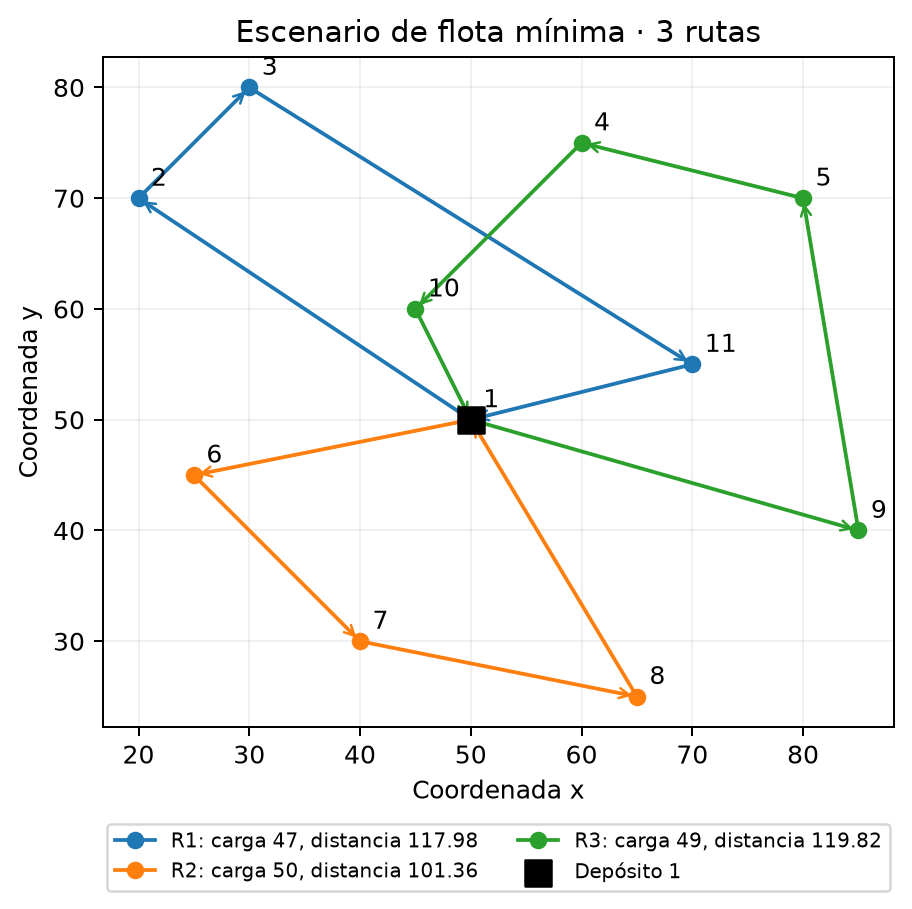
\includegraphics[width=0.82\linewidth,height=0.43\textheight,keepaspectratio]{figuras/rutas_tres.png}

\caption{Rutas óptimas para una flota de tres vehículos, con cargas de 47, 50 y 49 unidades.}\label{fig:3}

\end{figure}

La comparación muestra el compromiso entre distancia y tamaño de flota. Entre estos dos escenarios, la alternativa de tres vehículos conviene cuando el ahorro de un costo fijo por vehículo supera el costo de 20.175187 unidades adicionales de recorrido, conforme al marco económico de la sección 1.2.


\Needspace{110pt}

\subsection{Solución heurística}

\Needspace{130pt}

{\small\begin{longtable}{P{\dimexpr 0.07\linewidth-4.2pt\relax}P{\dimexpr 0.4\linewidth-24.000000000000004pt\relax}P{\dimexpr 0.19\linewidth-11.400000000000002pt\relax}P{\dimexpr 0.16\linewidth-9.6pt\relax}P{\dimexpr 0.18\linewidth-10.8pt\relax}}

\caption{Rutas de Clarke--Wright + 2-opt.}\label{tab:7}\\

\toprule

\textbf{Ruta} & \textbf{Recorrido} & \textbf{Distancia} & \textbf{Carga / 50} & \textbf{No utilizado}\\\midrule

\endfirsthead

\caption[]{Rutas de Clarke--Wright + 2-opt. (continuación)}\\

\toprule

\textbf{Ruta} & \textbf{Recorrido} & \textbf{Distancia} & \textbf{Carga / 50} & \textbf{No utilizado}\\\midrule

\endhead

\bottomrule\endfoot

R1 & 1 \(\to\) 11 \(\to\) 1 & 41.231 & 17 & 66\%\\[2pt]

R2 & 1 \(\to\) 3 \(\to\) 2 \(\to\) 6 \(\to\) 1 & 101.188 & 44 & 12\%\\[2pt]

R3 & 1 \(\to\) 7 \(\to\) 8 \(\to\) 1 & 77.011 & 36 & 28\%\\[2pt]

R4 & 1 \(\to\) 9 \(\to\) 5 \(\to\) 4 \(\to\) 10 \(\to\) 1 & 119.823 & 49 & 2\%\\[2pt]

\end{longtable}}

La heurística obtiene \(Z_H\) = 339.252870 unidades con cuatro rutas. Todas parten y terminan en el depósito, atienden una sola vez a cada cliente y respetan la capacidad. La capacidad libre global también es 27\%, pero está distribuida de otra manera: una ruta queda con 17 unidades y otra con 49. La igualdad en ocupación global no implica igualdad de recorrido.


\begin{figure}[H]\centering

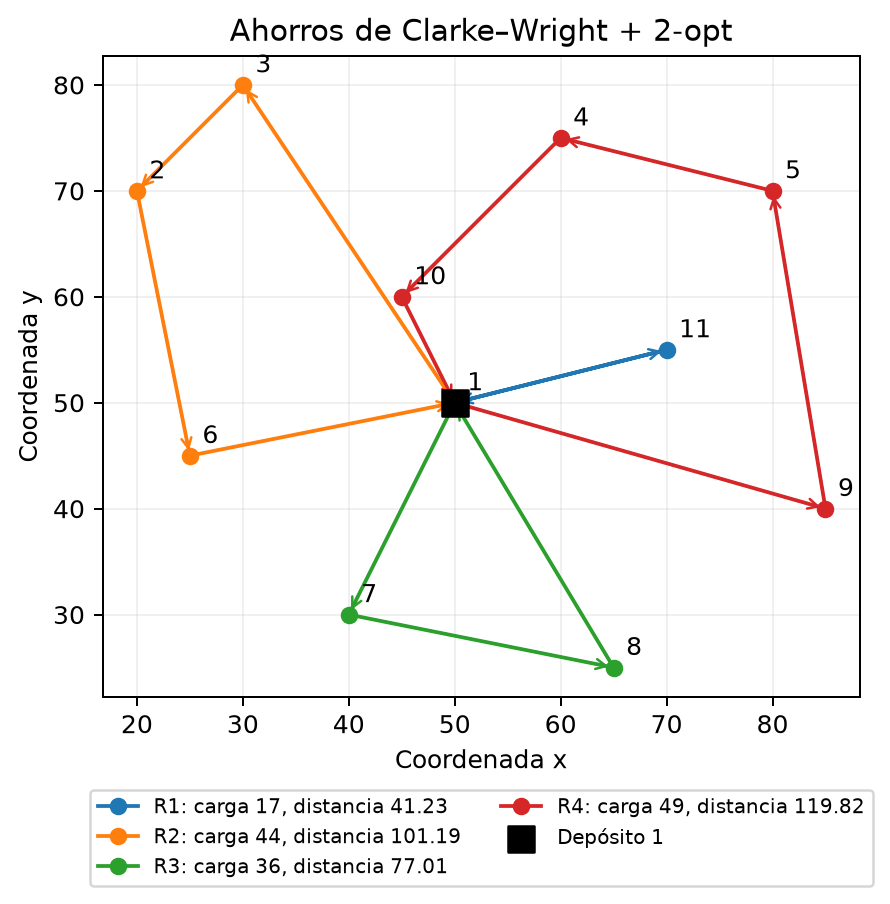
\includegraphics[width=0.82\linewidth,height=0.43\textheight,keepaspectratio]{figuras/rutas_heuristica.png}

\caption{Rutas obtenidas mediante Clarke--Wright + 2-opt.}\label{fig:4}

\end{figure}

La Figura~\ref{fig:4} conserva el grupo 3--2--6 de la solución exacta, pero deja al cliente 11 en una ruta individual y reúne 9--5--4--10 en otra. Estas asignaciones explican el mayor recorrido. La mejora 2-opt optimiza el orden dentro de cada ruta y conserva sus cargas; para modificar la agrupación sería necesario incorporar traslados o intercambios de clientes entre vehículos.


\Needspace{110pt}

\section{Comparación de calidad y tiempo}

\Needspace{110pt}

\subsection{Protocolo de medición}

Las mediciones se realizaron el 15 de octubre de 2026 en Windows 11, Python 3.12.10, PuLP 3.3.0 y CBC 2.10.3, con threads = 0 y tolerancias relativa y absoluta de brecha iguales a cero. Tras un calentamiento por escenario y de la heurística, se registraron diez ejecuciones sin flota fija y diez con exactamente tres rutas, con límite de 120 s por llamada al solver. La heurística se midió en las diez repeticiones del caso libre. El tiempo exacto comprende construcción del modelo, solución y reconstrucción de rutas; el heurístico comprende ahorros, fusiones y 2-opt. La lectura de datos, la matriz, la validación y las figuras se calcularon fuera del intervalo medido.


La Tabla~\ref{tab:8} recoge las mediciones individuales y la Tabla~\ref{tab:9} resume el caso sin flota fija mediante media, mediana y desviación estándar muestral. Las repeticiones corresponden a una misma instancia y permiten describir la variación temporal en este equipo.


\Needspace{270pt}

{\small\begin{longtable}{P{\dimexpr 0.14\linewidth-8.4pt\relax}P{\dimexpr 0.23\linewidth-13.8pt\relax}P{\dimexpr 0.2\linewidth-12.000000000000002pt\relax}P{\dimexpr 0.19\linewidth-11.400000000000002pt\relax}P{\dimexpr 0.24\linewidth-14.399999999999999pt\relax}}

\caption{Diez mediciones del modelo exacto y de la heurística, en milisegundos.}\label{tab:8}\\

\toprule

\textbf{Ejecución} & \textbf{Exacto libre total} & \textbf{CBC libre} & \textbf{Heurística} & \textbf{Exacto tres rutas}\\\midrule

\endfirsthead

\caption[]{Diez mediciones del modelo exacto y de la heurística, en milisegundos. (continuación)}\\

\toprule

\textbf{Ejecución} & \textbf{Exacto libre total} & \textbf{CBC libre} & \textbf{Heurística} & \textbf{Exacto tres rutas}\\\midrule

\endhead

\bottomrule\endfoot

1 & 3016.158 & 3013.264 & 0.107 & 10680.474\\[2pt]

2 & 3047.128 & 3044.389 & 0.213 & 11522.250\\[2pt]

3 & 2921.242 & 2917.696 & 0.117 & 11541.228\\[2pt]

4 & 2899.293 & 2895.761 & 0.354 & 11569.740\\[2pt]

5 & 3166.549 & 3160.588 & 0.295 & 10619.549\\[2pt]

6 & 2978.834 & 2973.297 & 0.202 & 11478.513\\[2pt]

7 & 2957.159 & 2952.768 & 0.192 & 11184.763\\[2pt]

8 & 2811.732 & 2808.970 & 0.122 & 11163.236\\[2pt]

9 & 2927.785 & 2924.961 & 0.222 & 10414.428\\[2pt]

10 & 3028.124 & 3024.541 & 0.159 & 9611.335\\[2pt]

\end{longtable}}

\Needspace{200pt}

{\small\begin{longtable}{P{\dimexpr 0.5\linewidth-18.0pt\relax}P{\dimexpr 0.25\linewidth-9.0pt\relax}P{\dimexpr 0.25\linewidth-9.0pt\relax}}

\caption{Resumen del modelo exacto y de la heurística sin flota fija.}\label{tab:9}\\

\toprule

\textbf{Indicador} & \textbf{Exacto} & \textbf{Heurística}\\\midrule

\endfirsthead

\caption[]{Resumen del modelo exacto y de la heurística sin flota fija. (continuación)}\\

\toprule

\textbf{Indicador} & \textbf{Exacto} & \textbf{Heurística}\\\midrule

\endhead

\bottomrule\endfoot

Distancia total & 318.989487 & 339.252870\\[2pt]

Rutas & 4 & 4\\[2pt]

Capacidad no utilizada & 27.00\% & 27.00\%\\[2pt]

Tiempo medio (ms) & 2975.400 & 0.198\\[2pt]

Desviación estándar del tiempo (ms) & 96.752 & 0.080\\[2pt]

Mediana (ms) & 2967.997 & 0.197\\[2pt]

GAP de costo respecto al óptimo & 0.00\% & 6.35\%\\[2pt]

\end{longtable}}


\begin{equation}\label{eq:gap}
\operatorname{GAP}_{Z}(\%)=100\,\frac{Z_H-Z^*}{Z^*}
\end{equation}


El GAP de costo obtenido es \(6.352\%\).


\begin{equation}\label{eq:tiempo}
R_t(\%)=100\,\frac{\overline t_E-\overline t_H}{\overline t_E}
\end{equation}


Las cantidades \(\overline t_E\) y \(\overline t_H\) son los tiempos medios del método exacto sin flota fija y de la heurística, expresados en la misma unidad.

La reducción temporal es 99.9933\%, calculada respecto del tiempo medio exacto. La diferencia porcentual con signo, tomando heurística menos exacto, es -99.9933\%.


La Figura~\ref{fig:5} compara la calidad y el tiempo de ambos métodos. La heurística recorre 20.263383 unidades adicionales, con GAP de 6.352\% respecto del óptimo. El método exacto tarda 2.975 s en promedio y la heurística 0.198 ms, una razón entre medias cercana a 15,008. La escala logarítmica del panel temporal permite representar esta diferencia de órdenes de magnitud. En esta instancia, la heurística ofrece una respuesta muy rápida a cambio de una distancia mayor; las magnitudes temporales dependen de la implementación y del equipo.


\begin{figure}[H]\centering

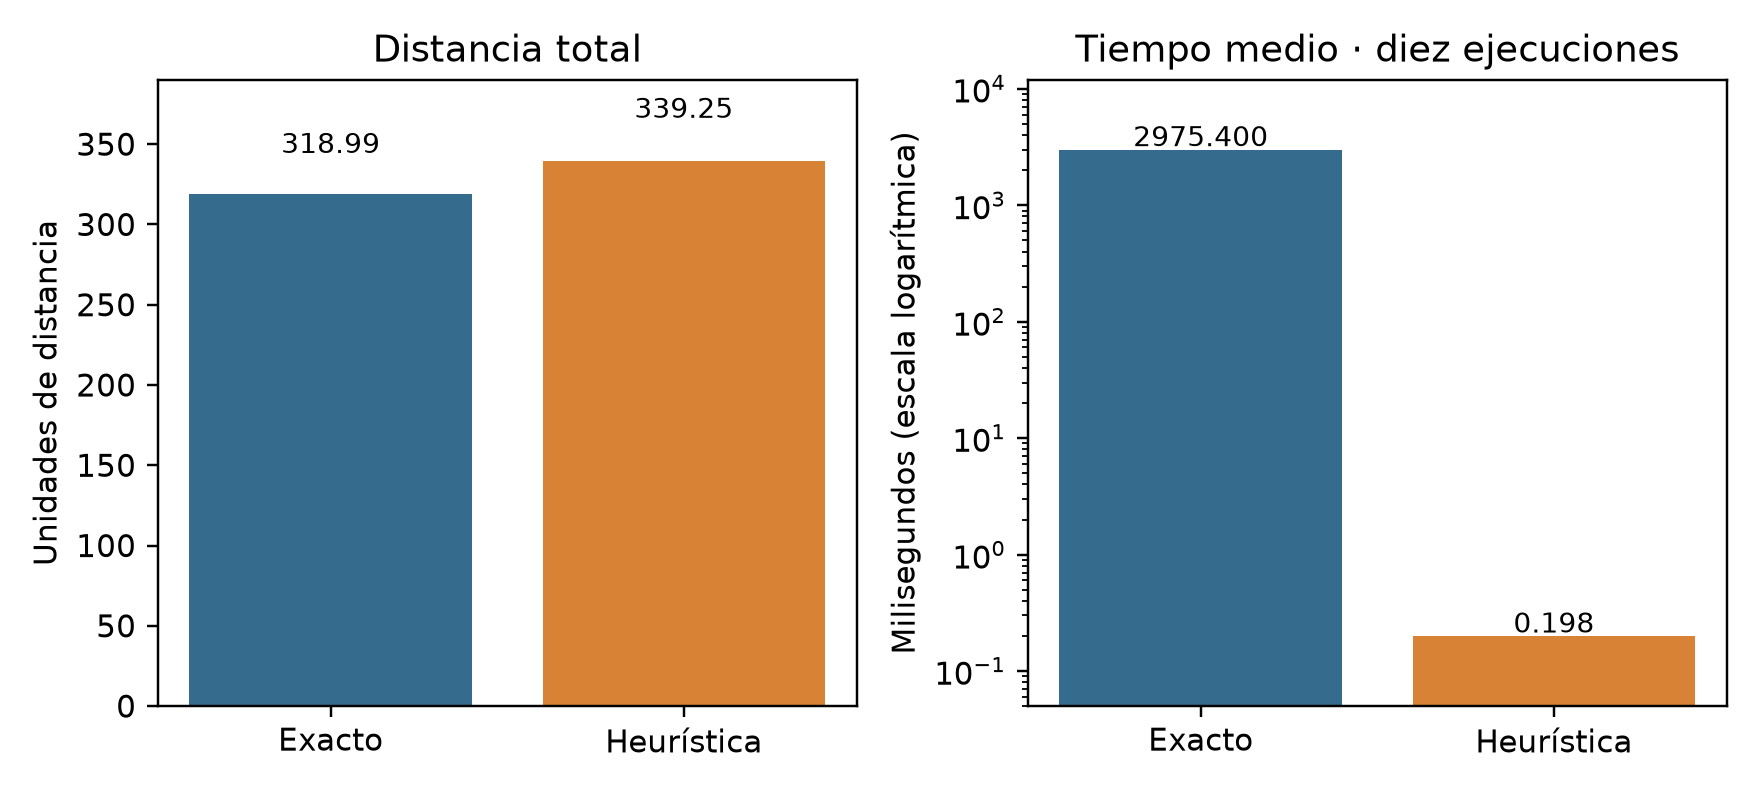
\includegraphics[width=1\linewidth,height=0.43\textheight,keepaspectratio]{figuras/comparacion.png}

\caption{Distancia y tiempo medio del método exacto y la heurística. Diez ejecuciones; tiempo en escala logarítmica.}\label{fig:5}

\end{figure}

En el caso sin flota fija, CBC registra 240 nodos de búsqueda y 20,066 iteraciones en cada ejecución. Con tres rutas, estos valores aumentan a 8,247 nodos y 204,300 iteraciones, y el tiempo medio llega a 10.979 \(\pm\) 0.641 s. La mayor exploración muestra que fijar la flota hace más exigente la resolución de esta instancia.


\Needspace{110pt}

\subsection{Comparación independiente de formulaciones}

Para evaluar el efecto de la formulación, se compararon tres variantes: A añade al modelo de flujo restricciones explícitas de eliminación de subrutas; B es la formulación principal de la sección 4; C refuerza B con las cotas \(q_jx_{ij}\le f_{ij}\le(Q-q_i)x_{ij}\). La variante A incluye 1,013 restricciones por subconjuntos de clientes y tiene 1,167 restricciones en total; B tiene 154 y C, 264. Las tres describen las mismas soluciones enteras factibles para esta instancia.


Esta comparación empleó diez repeticiones, un calentamiento por variante y escenario, orden rotado A/B/C y límite de 120 s por ejecución. Sin flota fija, los tiempos medios fueron 5.49 s, 2.07 s y 1.78 s para A, B y C, respectivamente, con optimalidad probada en todas las corridas. Con tres rutas, B y C probaron el óptimo en diez de diez ejecuciones y tardaron 17.4 s y 23.4 s en promedio. A lo probó en dos de diez y consumió 113.5 s en promedio, incluyendo las corridas detenidas por tiempo. La formulación compacta fue favorable en estos ensayos, mientras que reforzar sus cotas no mejoró ambos escenarios. Este experimento se analiza por separado de la medición principal de la sección 7.1.


\Needspace{110pt}

\section{Relación con el reparto urbano y métodos bioinspirados}

La situación permite formular decisiones de ruteo, asignación de carga, horarios, localización de puntos de entrega y selección de flota. El CVRP aborda las dos primeras. Las ventanas de tiempo permitirían representar horarios de acceso; los tiempos de viaje dependientes de la hora representarían congestión; los costos de espera y servicio incorporarían parte de la dificultad de estacionamiento. Los casilleros y centros logísticos requieren decisiones adicionales de localización y asignación, no sólo reordenar rutas.


Para un CVRP de mayor tamaño se propone evaluar un algoritmo genético híbrido, respaldado por los enfoques de Prins (2004) y Vidal (2022): una permutación representa clientes, un procedimiento de división construye rutas y una búsqueda local mejora la solución. El trabajo de Orrego Cardozo et al. (2016) ofrece otra combinación de barrido y evolución. Son candidatos apropiados cuando el espacio de soluciones impide una enumeración completa; su calidad debe medirse contra referencias exactas pequeñas o mejores soluciones conocidas, con varias semillas y límites de tiempo comparables.


Si se desea mejorar simultáneamente costo, puntualidad y emisiones, primero se distinguirían restricciones obligatorias ---capacidad y atención de todos los clientes--- de criterios negociables. Después se podrían comparar soluciones no dominadas o emplear un objetivo ponderado con escalas normalizadas y pesos justificados. El ejemplo de tres frente a cuatro rutas ya exhibe un compromiso entre recorrido y utilización. Para decidir entre camiones, bicicletas o vehículos eléctricos habría que añadir capacidades, autonomía, accesibilidad, recarga y costos propios de cada tipo.


\Needspace{110pt}

\section{Conclusiones}

La instancia requiere al menos tres rutas y puede atenderse con esa flota, pero la menor distancia se alcanza con cuatro rutas y 318.989487 unidades. Con tres vehículos, la distancia sube a 339.164674 unidades: un incremento de 6.325\% acompañado de mayor utilización de capacidad. La elección operativa depende, por tanto, del costo fijo de los vehículos y del valor asignado al recorrido.


Clarke--Wright + 2-opt produce una solución factible de 339.252870 unidades, con GAP de 6.352\%. Su tiempo medio de 0.198 ms, frente a 2.975 s del modelo exacto, muestra su utilidad como procedimiento rápido para esta instancia. El modelo de flujo permite representar explícitamente recorridos, cargas, visitas y capacidad, y certificar la calidad de la solución heurística. Como siguiente etapa se propone incorporar mejoras entre rutas y evaluar varias instancias antes de extender el análisis a congestión, horarios y emisiones.


\clearpage

\section*{Referencias}

{\small\hangindent=1.2em\hangafter=1 Bekta\c{s}, T., \& Laporte, G. (2011). The Pollution-Routing Problem. Transportation Research Part B: Methodological, 45\eqref{eq:m8}, 1232--1250. \href{https://doi.org/10.1016/j.trb.2011.02.004}{10.1016/j.trb.2011.02.004}\par}

{\small\hangindent=1.2em\hangafter=1 Clarke, G., \& Wright, J. W. (1964). Scheduling of Vehicles from a Central Depot to a Number of Delivery Points. Operations Research, 12\eqref{eq:m4}, 568--581. \href{https://doi.org/10.1287/opre.12.4.568}{10.1287/opre.12.4.568}\par}

{\small\hangindent=1.2em\hangafter=1 Dalla Chiara, G., \& Goodchild, A. (2020). Do commercial vehicles cruise for parking? Empirical evidence from Seattle. Transport Policy, 97, 26--36. \href{https://doi.org/10.1016/j.tranpol.2020.06.013}{10.1016/j.tranpol.2020.06.013}\par}

{\small\hangindent=1.2em\hangafter=1 Gillett, B. E., \& Miller, L. R. (1974). A Heuristic Algorithm for the Vehicle-Dispatch Problem. Operations Research, 22\eqref{eq:m2}, 340--349. \href{https://doi.org/10.1287/opre.22.2.340}{10.1287/opre.22.2.340}\par}

{\small\hangindent=1.2em\hangafter=1 Material de la actividad. (s. f.). NAME \_CVRP\_10\_manual.txt [Instancia didáctica CVRP\_10 de diez clientes]. Archivo proporcionado para este reto.\par}

{\small\hangindent=1.2em\hangafter=1 McKinsey \& Company. (2016). Parcel delivery: The future of last mile (p. 6). \href{https://www.mckinsey.com/~/media/mckinsey/industries/travel\%20transport\%20and\%20logistics/our\%20insights/how\%20customer\%20demands\%20are\%20reshaping\%20last\%20mile\%20delivery/parcel_delivery_the_future_of_last_mile.pdf}{Documento fuente}\par}

{\small\hangindent=1.2em\hangafter=1 McKinsey \& Company. (2018). Technology delivered: Implications for cost, customers, and competition in the last-mile ecosystem. \href{https://www.mckinsey.com/industries/logistics/our-insights/technology-delivered-implications-for-cost-customers-and-competition-in-the-last-mile-ecosystem}{Documento fuente}\par}

{\small\hangindent=1.2em\hangafter=1 Orrego Cardozo, J. P., Ospina Toro, D., \& Toro Ocampo, E. M. (2016). Solución al Problema de Ruteo de Vehículos con Capacidad Limitada (CVRP) usando una técnica metaheurística. Scientia et Technica, 21\eqref{eq:m3}, 225--233. \href{https://doi.org/10.22517/23447214.9013}{10.22517/23447214.9013}\par}

{\small\hangindent=1.2em\hangafter=1 Prins, C. (2004). A simple and effective evolutionary algorithm for the vehicle routing problem. Computers \& Operations Research, 31(12), 1985--2002. \href{https://doi.org/10.1016/S0305-0548(03)00158-8}{10.1016/S0305-0548(03)00158-8}\par}

{\small\hangindent=1.2em\hangafter=1 Reinelt, G. (1991). TSPLIB---A Traveling Salesman Problem Library. ORSA Journal on Computing, 3\eqref{eq:m4}, 376--384. \href{https://doi.org/10.1287/ijoc.3.4.376}{10.1287/ijoc.3.4.376}\par}

{\small\hangindent=1.2em\hangafter=1 Reinelt, G. (s. f.). TSPLIB FAQ. Universität Heidelberg. \href{https://comopt.ifi.uni-heidelberg.de/software/TSPLIB95/tsp/TSPFAQ.html}{Documento fuente}\par}

{\small\hangindent=1.2em\hangafter=1 Sherman, N. (2018, 4 de enero). Crowded streets: Cities face a surge in online deliveries. BBC News. \href{https://www.bbc.com/news/business-42245367}{Documento fuente}. Referencia contextual proporcionada en la situación problema del curso.\par}

{\small\hangindent=1.2em\hangafter=1 Toth, P., \& Vigo, D. (Eds.). (2014). Vehicle Routing: Problems, Methods, and Applications (2.\textsuperscript{a} ed.). SIAM. \href{https://doi.org/10.1137/1.9781611973594}{10.1137/1.9781611973594}\par}

{\small\hangindent=1.2em\hangafter=1 tsplib95. (s. f.). tsplib95.distances: euclidean. Documentación de la versión 0.7.1. \href{https://tsplib95.readthedocs.io/en/stable/_modules/tsplib95/distances.html}{Documento fuente}\par}

{\small\hangindent=1.2em\hangafter=1 Vidal, T. (2022). Hybrid genetic search for the CVRP: Open-source implementation and SWAP* neighborhood. Computers \& Operations Research, 140, 105643. \href{https://doi.org/10.1016/j.cor.2021.105643}{10.1016/j.cor.2021.105643}\par}

{\small\hangindent=1.2em\hangafter=1 World Economic Forum. (2020). The Future of the Last-Mile Ecosystem (pp. 5 y 21). \href{https://www3.weforum.org/docs/WEF_Future_of_the_last_mile_ecosystem.pdf}{Documento fuente}\par}

{\small\hangindent=1.2em\hangafter=1 Zhang, J., Zhao, Y., Xue, W., \& Li, J. (2015). Vehicle routing problem with fuel consumption and carbon emission. International Journal of Production Economics, 170, 234--242. \href{https://doi.org/10.1016/j.ijpe.2015.09.031}{10.1016/j.ijpe.2015.09.031}\par}

\clearpage

\appendix

\section{Código de solución}

El código completo, la instancia y los resultados se encuentran en \href{https://github.com/Leo-issacs/cvrp-logistica-urbana}{el repositorio del proyecto}. Los siguientes extractos muestran la construcción del modelo y la heurística. Las opciones A, B y C corresponden a las variantes definidas en la sección 7.2; B selecciona la formulación principal.


\begin{minipage}{\linewidth}

\begin{lstlisting}

python src/resolver_cvrp_arcos.py data/instancia.txt \
    --modelo B --out results/nueva_ejecucion

\end{lstlisting}

\end{minipage}

La función construir\_modelo genera las variables de recorrido y carga, la función objetivo y las restricciones. Utiliza math, itertools como it, PuLP y el diccionario MODELOS del módulo. El parámetro fixed\_k permite fijar el número de rutas.


\begin{lstlisting}[language=Python]

def construir_modelo(q,Q,depot,d,modelo='B',fixed_k=None):
    """Modelo de arcos x y carga fisica f. modelo: A, B o C (ver MODELOS).
    Eliminar las subrutas explicitas (B, C) es valido solo si toda demanda de cliente es
    positiva: sumando el balance de producto (5) sobre un conjunto aislado S los flujos
    internos se cancelan y queda 0 = suma de q_i en S > 0, imposible. Con una demanda nula
    un ciclo aislado de clientes sin demanda seria factible: en ese caso se exige modelo A."""
    if modelo not in MODELOS: raise ValueError(f'modelo desconocido: {modelo}')
    V=sorted(q); C=[i for i in V if i!=depot]
    if modelo!='A' and any(q[i]<=0 for i in C):
        raise ValueError('el modelo '+modelo+' requiere demandas de clientes positivas; use el modelo A (con subrutas)')
    A=[(i,j) for i in V for j in V if i!=j]
    model=pulp.LpProblem('CVRP_arcos_carga',pulp.LpMinimize)
    x=pulp.LpVariable.dicts('x',A,cat='Binary')
    f=pulp.LpVariable.dicts('f',A,lowBound=0)
    model += pulp.lpSum(d[i,j]*x[i,j] for i,j in A), 'distancia'
    for i in C:
        model += pulp.lpSum(x[j,i] for j in V if j!=i)==1, f'visita_{i}'
        model += pulp.lpSum(x[i,j] for j in V if j!=i)==pulp.lpSum(x[j,i] for j in V if j!=i), f'continuidad_{i}'
        model += pulp.lpSum(f[j,i] for j in V if j!=i)-pulp.lpSum(f[i,j] for j in V if j!=i)==q[i], f'entrega_{i}'
        model += f[i,depot]==0, f'regreso_vacio_{i}'
    m=pulp.lpSum(x[depot,j] for j in C)
    model += m==pulp.lpSum(x[i,depot] for i in C), 'balance_deposito'
    model += m>=math.ceil(sum(q.values())/Q), 'flota_minima_cota'
    model += m<=len(C), 'flota_maxima'
    model += pulp.lpSum(f[depot,j] for j in C)==sum(q.values()), 'carga_inicial_total'
    if fixed_k is not None: model += m==fixed_k, 'flota_fija'
    for i,j in A:
        if modelo=='C':
            model += f[i,j]<=(Q-q[i])*x[i,j], f'capacidad_{i}_{j}'
            model += f[i,j]>=q[j]*x[i,j], f'carga_minima_{i}_{j}'
        else:
            model += f[i,j]<=Q*x[i,j], f'capacidad_{i}_{j}'
    n_sec=0
    if modelo=='A':
        for size in range(2,len(C)+1):
            for S in it.combinations(C,size):
                model += pulp.lpSum(x[i,j] for i in S for j in S if i!=j)<=len(S)-1, f'subtour_{n_sec}'
                n_sec+=1
    return model,x,f,A,C,n_sec


\end{lstlisting}

La heurística usa ahorros de Clarke--Wright y mejora 2-opt dentro de cada ruta. Estas funciones emplean costo(ruta, d), definida como la suma de distancias entre nodos consecutivos, e itertools como it.


\clearpage

\begin{lstlisting}[language=Python]

def costo(route,d): return sum(d[a,b] for a,b in zip(route,route[1:]))


def dos_opt(route,d):
    while True:
        best=route; bestcost=costo(route,d)
        for a in range(1,len(route)-2):
            for b in range(a+1,len(route)-1):
                candidate=route[:a]+list(reversed(route[a:b+1]))+route[b+1:]
                z=costo(candidate,d)
                if z < bestcost-1e-10: best,bestcost=candidate,z
        if best is route: return route
        route=best


def heuristica(q,Q,depot,d):
    clients=sorted(set(q)-{depot}); routes=[[i] for i in clients]
    savings=sorted(((d[depot,i]+d[depot,j]-d[i,j],i,j)
                    for i,j in it.combinations(clients,2)),key=lambda t:(-t[0],t[1],t[2]))
    for s,i,j in savings:
        if s<=0: continue
        a=next(r for r in routes if i in r); b=next(r for r in routes if j in r)
        if a is b or i not in (a[0],a[-1]) or j not in (b[0],b[-1]): continue
        if sum(q[v] for v in a+b)>Q: continue
        aa=a if a[-1]==i else a[::-1]; bb=b if b[0]==j else b[::-1]
        routes.remove(a); routes.remove(b); routes.append(aa+bb)
    return [dos_opt([depot]+r+[depot],d) for r in routes]


\end{lstlisting}

El programa verifica la cobertura de clientes, la capacidad y la continuidad de las rutas. La clasificación del solver distingue optimalidad probada de una solución factible obtenida al alcanzar el límite de tiempo. La certificación por particiones se realiza fuera del intervalo usado para medir el tiempo de solución.


\end{document}